\documentclass[10pt]{exam}
\usepackage[hon]{template-for-exam}
\usepackage{tikz}
\usetikzlibrary{shadings,decorations.pathmorphing,arrows.meta,patterns}

\title{Superposition in Coulomb's Law}
\author{Rohrbach}
\date{\today}

\begin{document}
\maketitle

\noindent
Three point charges $q_1$, $q_2$, and $q_3$ lie along the $x$-axis at $x=-0.4$ m, $0$ m, and $1.0$ m, respectively.  Calculate the magnitude and direction of electrostatic force on charge $q_3$ when
%
\begin{align*}
q_1 &=+\SI{1.3e-5}{\coulomb}\, ,  \\
q_2 &=-\SI{6.0e-5}{\coulomb}\, \text{, and} \\
q_3 &=-\SI{5.7e-5}{\coulomb}\, .
\end{align*} 

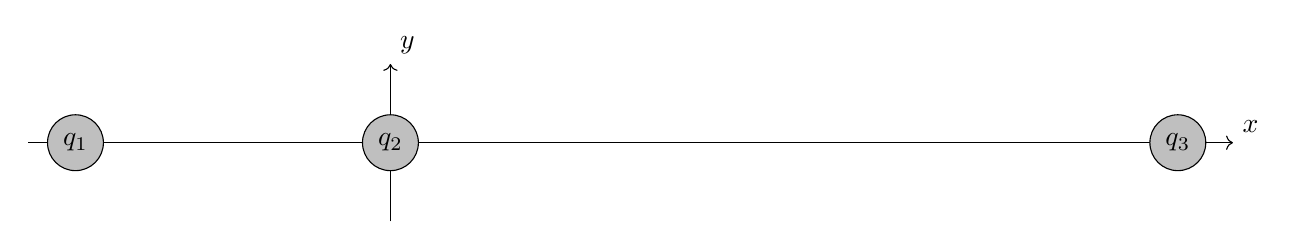
\begin{tikzpicture}
  \draw[->] (0,-1) -- (0,1) node[anchor=south west] {$y$};
  \draw[->] (-4.6,0) -- (10.7,0) node[anchor=south west] {$x$};


  \node[shape=circle,draw,fill=gray!50] at (-4,0) {$q_1$};
  \node[shape=circle,draw,fill=gray!50] at ( 0,0) {$q_2$};
  \node[shape=circle,draw,fill=gray!50] at (10,0) {$q_3$};

\end{tikzpicture}




\end{document}